\section{Historia de la Empresa}
Elevadores H\'{e}rcules S.A., se estableci\'{o} en Buenos Aires en 1919 como una oficina de contratistas.
Su planta principal est\'{a} ubicada en Buenos Aires. Adem\'{a}s tiene oficinas comerciales en las 18 ciudades m\'{a}s importantes del pa\'{i}s participando con m\'{a}s del 60 \% del mercado nacional.

\subsection{Avance Cronol\'{o}gico de la empresa}
\begin{enumerate}
	\item \underline{1966}. La compa\~{n}\'{i}a produc\'{i}a 1650 elevadores. 
	\item \underline{1970}. Hacia esta d\'{e}cada el n\'{u}mero de edificios comenz\'{o} a aumentar considerablemente. Los pedidos de los clientes tend\'{i}an a sobrepar la capacidad de producci\'{o}n de la f\'{a}brica.
	\item \underline{1974}. Lleg\'{o} a producir 7.850 unidades, inclusive escaleras mec\'{a}nicas.
\end{enumerate}

\section{Resumen del Funcionamiento}

\subsection{Caracter\'{i}sticas del Sistema de Producci\'{o}n}
\begin{itemize}
	\item \emph{No} depende de proveedores para la fabricaci\'{o}n de los productos, es decir, la misma es vertical. La empresa no terceriza nada sino que todo lo produce ella misma. Con lo cual toda la producci\'{o}n es propia.
	\item Producci\'{o}n diversificada debido a lo anterior, dando lugar a un complejo sistema de producci\'on en general.
	\item Producci\'{o}n no estandarizada, debido a los diversos requerimientos de los clientes. Cuenta con pocas piezas estandarizadas.
	\item El planeamiento tambi\'{e}n est\'a dificultado por el desarrollo tecnol\'ogico de la construcci\'on de diferentes lugares, dependiendo as\'i de condiciones que no se pueden preveer. Al producir todo la misma empresa el planeamiento se torna dificultoso, ya que no solamente se construye el elevador sino que tambien se tienen que construir todas las piezas del mismo, lo que hace que la planificaci\'{o}n tambi\'{e}n incluya la construcci\'{o}n de las piezas. Otro punto que dificulta el planeamiento es que los procesos no cuentan con una adecuada estandarizaci\'{o}n. Por lo tanto, frente a cada uno de los pedidos que van ingresando es necesario hacer una planificaci\'{o}n completamente nueva, lo cual aumenta el margen de error aumentando la ineficiencia.
	\item Equipo de producci\'{o}n y montaje dividido en 4 grupos(seg\'{u}n la secuencia en el orden de entrega de partes.)
	\item Producci\'{o}n organizada por secciones:
	\begin{enumerate}
		\item M\'{a}quinas operativas.
		\item Estampado.
		\item Montaje de m\'{a}quinas.
		\item Montaje de motores
		\item Montaje de aparatos el\'{e}ctricos.
		\item Montaje y conexi\'{o}n de cuadros de comando.
		\item Carpinter\'{i}a, fabricaci\'{o}n de contrapesos, cabinas y 	puertas de acero.
		\item Carpinter\'ia, cabinas, puertas y plataformas de madera.
		\item Pintura y galvanoplast\'ia.
	\end{enumerate}
	\item Proceso de Planeamiento de Producci\'{o}n
	\begin{itemize}
		\item El equipo de producci\'{o}n y montaje de elevadores estaba formado en grupos.
		\item Cada grupo responsable de una tarea diferente.
		\item El Jefe de grupo estimaba futuras necesidades, volcando esto en un formulario de avances del mes, donde planificaba adem\'{a}s tiempos de entrega seg\'{u}n el proceso de producci\'{o}n mencionado antes.
		\item  Se entregaba el formulario a un asistente(planeador) del Departamento de Producci\'{o}n.
		\item El planeador con dichos formularios, elabora el programa de producci\'{o}n siguiendo una secuencia impuesta por el Departamento de Ventas(orden de entrada de los pedidos de los clientes)
		\item El planeador tambi\'{e}n recibe ordenes de fabricaci\'{o}n individuales del Departamento de Ingenier\'{i}a, que contiene las especificaciones para producir el elevador.
	\end{itemize}
	\item Cuando la cantidad de elevadores producidos era baja comparada con la capacidad de producci\'{o}n el planeamiento era simple,eficaz y de f\'{a}cil control. 
	\item Hacia 1970, los retrasos en las entregas hacian que:
	\begin{itemize}
		\item Jefes de campo fijaran plazos muy anticipados, haciendole perder el valor agregado del programador.
		\item Falla en la comunicaci\'{o}n al momento de la par\'{a}lisis de las obras de un edificio, produciendo estancamiento de stock y as\'{i} generando grandes atrasos y malestar de los clientes.
		\item Por todo esto el Departamento de Ventas sugiri\'{o} cambios en las prioridades de las ordenes de producci\'{o}n
		\item Se abandon\'{o} la programaci\'{o}n que se llevaba hasta ese momento, dependiendo de las ordenes de venta del Departamento respectivo.
	\end{itemize}
\end{itemize}

\newpage
\section{Organigrama tentativo}
Se detalla un organigrama parcial que se confecciona a partir de la informaci\'on proporcionada en la descripci\'on del caso.

\begin{figure}[H]
\centering
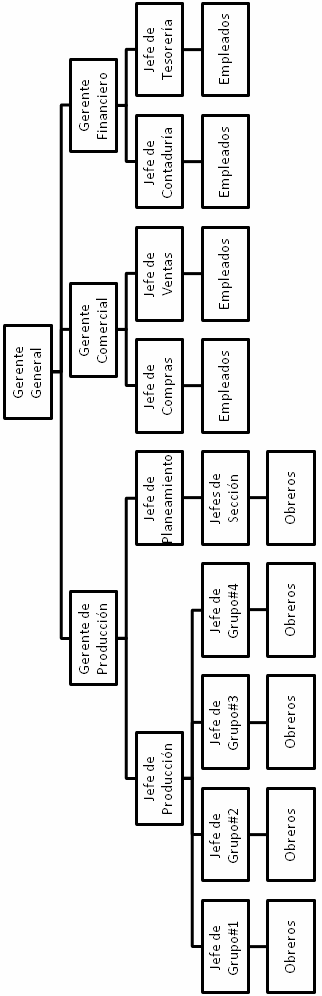
\includegraphics[scale=0.75]{images/organigrama-hercules.png}
\end{figure}

\newpage
\section{An\'{a}lisis del caso}

\subsection{Marco Te\'orico}

\subsubsection{Tipo de empresa}
La empresa fue en sus comienzos probablemente una PyME, y a medida que aument\'o su tama\~no desarroll\'o su vida como una sociedad civil. En este sentido, si bien nunca fue una empresa familiar, su estructura y organizaci\'on iniciales fueron evolucionando gradualmente a lo que es en la actualidad, probablemente provocando los problemas de planeamiento observados. Es decir, si una empresa no sufre un proceso formal de dise\~no organizacional, es altamente probable que se encuentren deficiencias en su funcionamiento a medida que pasa el tiempo y aumenta su tama\~no. Por este motivo resulta conveniente la reestructuraci\'on que se propone la empresa al contratar una consultora.

\subsubsection{Proceso de creaci\'on de valor}
Una observaci\'on interesante es el amplio proceso de conversi\'on de insumos en productos. La empresa toma como insumos materias primas muy esenciales, para utilizar en fundici\'on, carpinter\'ia, torner\'ia, moldeado, rectificaci\'on, montaje, pintura, estampado y la final instalaci\'on de los productos. Una empresa de esta complejidad necesita una estructura s\'olida y una programaci\'on muy precisa para funcionar eficientemente.

\subsubsection{Rasgos de pensamiento administrativo}
Evidentemente la empresa evolucion\'o hacia el modelo de Taylor: en un principio delegaba en los empleados parte del planeamiento de producci\'on, quienes reportaban al planeador de producci\'on, que luego completaba la programaci\'on. Esto trajo problemas por dos motivos; uno de ellos los errores de relevamiento de dichos empleados, quienes omit\'ian reportar obras paralizadas y fijaban plazos de entrega muy anticipados para tratar de compensar los retrasos en las entregas (meti\'edose en una parte de la organizaci\'on que no era su responsabilidad); el otro motivo fue el aumento de la demanda, que hizo imposible continuar con este precario sistema. Se pasa entonces a trabajar seg\'{u}n ordenes de venta, lo cual hace el negocio menos previsible (quita la posibilidad de reaccionar ante fluctuaciones en el mercado, la programaci\'on se hace a medida que se vende pero no se pronostica la potencial demanda futura).

\subsection{Problema principal de la empresa}
\subsubsection{La empresa no puede enfrentar al cambio en el mercado}
El problema principal de H\'ercules surge al producirse un cambio en el mercado. La empresa comienza atendiendo a una cantidad de clientes con la cual puede trabajar en forma eficiente y c\'omoda. Al empezar a irle bien cada vez cuenta con m\'as clientes y m\'as pedidos. Esto deber\'ia serle algo muy positivo a la misma, ya que le implicar\'ia ganar m\'as que antes y ampliar su mercado. Pero esto no es lo que sucede ya que, contrario a lo que se supone como un crecimiento, es aqu\'i cuando empiezan los problemas.\\

\subsection{Consecuencias del problema principal de la empresa y sus propuestas de soluci\'on}

\subsubsection{No hay una determinaci\'on de que procesos dan valor y cuales no}
La empresa es dif\'icil de controlar y no logra una correcta planificaci\'on, debido a que su proceso productivo es muy amplio y abarcativo. De un an\'alisis de los procesos industriales de la empresa puede reconocerse una falencia: hay procesos que no agregan valor al producto final. Es decir, la empresa realiza tareas como la fabricaci\'on de las piezas a utilizar en la construcci\'on de los elevadores, las cuales podr\'ian ser compradas a terceros. Como se mencionar\'a m\'as adelante, la fabricaci\'on de las piezas tambi\'en representa un costo innecesario.
\paragraph{Soluci\'on}
Se debe determinar qu\'e procesos que agregan valor y los que no. A partir de all\'i tomar decisiones en la direcci\'on de abandonar los procesos que no producen un beneficio a la empresa, ya sea directo o indirecto (ventajas competitivas, por ejemplo), y si este beneficio justifica el costo del proceso. Un claro ejemplo de proceso que agrega valor en la empresa es el dise\~no y construcci\'on de elevadores. Este es un trabajo que la empresa transforma directamente en ingresos, ya que es su actividad principal. Un ejemplo de proceso que no agrega valor es el de la fabricaci\'on de piezas est\'andar: ellas pueden ser compradas a un tercero, y probablemente adem\'as se reduzca su costo, ya que el tercero puede producirla en mayor cantidad, y la empresa deber\'ia poder abandonar los costos fijos asociados a su producci\'on.

\subsubsection{Grave problema de costos}
La empresa tiene un grave problema de costos, algunos de ellos ocultos tras otros problemas. Se encuentra desbordada de pedidos y no tiene una respuesta eficiente; para intentar hacerles frente a los mismos toma decisiones equivocadas y principalmente apresuradas. Intentar vender m\'as en este caso no le esta garantizando mayor ganancia ya que en alg\'un momento esta situaci\'on de toma de decisiones erroneas va a hacer que el rendimiento comience a bajar notoriamente. Las principales decisiones erroneas son:
	\begin{itemize}
 		\item Coloca personal incapacitado para ciertos puestos. 
		\item No tiene un control efectivo de lo que produce, puede estar produciendo piezas equivocadas o m\'as de lo que realmente necesita ya que no cuenta con un plan eficaz. Esto se traduce en un costo de almac\'en porque debe acumular stock de piezas.
		\item Acepta cualquier pedido sin saber si realmente llega a cumplimentarlo, por una descoordinaci\'on entre el \'area de ventas y el \'area de producci\'on.
		\item Construye cada elevador a medida del cliente lo cual perjudica la producci\'on ya que no est\'a estandarizada, lo cual hace que aumente el margen de error (costos de reparaci\'on y/o reemplazo), agrega un costo de dise\~no a cada proyecto, agrega un costo de servicio de venta personalizado, etc.
	\end{itemize}
\paragraph{Soluci\'on}
Para el problema de costos una posible soluci\'on es estandarizar los procesos de producci\'on, y establecer un nuevo proceso de selecci\'on de personal, al menos del jer\'arquico.\\
Deben dise\~narse una serie de modelos est\'andar determinando antes cu\'ales son las caracter\'isticas de los elevadores m\'as vendidos, armar un catalogo para ofrecer a los clientes y fabricar los productos en serie. De esta manera es posible disminuir al menos dos costos: el de dise\~no, que no debe repetirse para cada cliente, y el de producci\'on o compra de piezas, ya que se estandarizar\'an completamente. Con esto podr\'ia llegar a perder una parte del mercado, pero consideramos que no ser\'{a} una gran parte ya que los productos a medida en general son m\'as costosos que los est\'andar, y los productos menos costosos son los que consiguen mayor caudal de ventas.\\
Se propone que el proceso de fabricaci\'on de piezas sea tercerizado, con esto bajar\'a la dificultad del planeamiento, se tendr\'{a} un menor sector de producci\'on m\'{a}s controlable, m\'as eficiente. Disminuir\'an notablemente los costos de dep\'osito, el costo de la planificaci\'on, se reducir\'a tambi\'en el costo de las piezas, ya que al ser est\'andar habr\'a m\'as de un proveedor compitiendo con sus precios por abastecer a la empresa.\\
Para lograr este tipo de decisiones debe contratarse personal capacitado para la planificaci\'on de una empresa de la escala de H\'ercules, si es posible con experiencia en el \'area de las instalaciones en la construcci\'on, por lo menos un director o gerente de planeamiento de producci\'on que posea mayores conocimientos que los t\'ecnicos de este \'area, para poder ejercer una autoridad real. Puede establecerse un \'area de recursos humanos para definir pol\'iticas de reclutamiento apuntadas a este objetivo, o contratarse una agencia consultora de forma temporal si no se requieren tareas de RR.HH. continuas.

\subsubsection{Falta de estandarizaci\'on, diversidad de productos}
La empresa se maneja en un ambiente muy cambiante, donde las variables externas (que no son controlables) son abundantes: los productos no son est\'andar, por ello no hay plan general de producci\'on (por la particularidad de cada producto vendido); el desarrollo tecnol\'ogico de la construcci\'on var\'ia segn el lugar de instalaci\'on de cada productos, etc.
\paragraph{Soluci\'on}
La empresa necesita un vuelco hacia el enfoque de contingencias, para adaptar las variables administrativas a las externas (que no son controlables.) En este sentido, se debe verificar que el personal administrativo cuente con el alcance temporal de la discreci\'on adecuado. Se debe adem\'{a}s analizar el ambiente externo produciendo informaci\'on confiable para reducir el riesgo en la toma de decisiones. Por ejemplo, contratar una consultora, o abrir una nueva \'area de la empresa, dedicada a la estad\'istica y pron\'osticos de mercado.

\subsubsection{Contrataci\'on de personal no capacitado para las tareas requeridas}
Se nombr\'o a cargo del Planeamiento de la Producci\'on a un antiguo supervisor en 1942. El nombramiento de esta persona no cumple con los requisitos del alcance temporal de la discreci\'on. Esto quiere decir que la persona no tiene la capacidad de predecir o anticipar el desarrollo de la tarea en el lapso de tiempo adecuado para tomar decisiones de planeamiento. Esto se ve reflejado en el siguiente parrafo de la descripci\'on del caso: "Los retrasos en las entregas de elevadores hicieron que los jefes de campo fijasen los plazos de entrega muy anticipados en sus informes mensuales. Con eso las informaciones recibidas por el programador, fueron perdiendo parte de su valor como base para la programaci\'on."\ Al poner personas en lugares equivocados no se soluciona nada sino que se empeora la situaci\'on. La empresa quiza quiera ahorrarse alg\'un costo de traer a un profesional, pero a la larga el costo ser\'a mayor por no hacerlo.
\paragraph{Soluci\'on}
Se propone situar en ese cargo a una persona que cumpla con los requerimientos que la posici\'on requiere. Alguien con experiencia y previsi\'on, que sea capaz de coordinar tiempos y tareas junto con el Area de Produccion.

\subsubsection{Conflictos entre algunas \'areas de la empresa}
"Los pedidos de los clientes tend\'ian a alcanzar l\'imites que sobrepasaban la capacidad de producci\'on de la f\'abrica. Los atrasos en la entrega de pedidos llegaron al punto de provocar serios conflictos entre los departamentos de ventas y producci\'on."
\paragraph{Soluci\'on}
Se propone incluir alg\'un tipo de nexo entre ambos departamentos. No puede pasar que el departamento de ventas y de producci\'on no se comuniquen ya que lo que se produce es lo que se vende, no se puede vender algo que no se va a poder producir. La gente de ventas no tiene el m\'as m\'inimo conocimiento de como se produce (lo cual es correcto ya que su funci\'on no es producir, sino vender) por lo que no tiene una noci\'on exacta de tiempos. Por lo que si no hay alguien que actue de nexo entre ambas \'areas, nunca va a funcionar bien. Encima una empresa vive de lo que vende por lo que este es un punto realmente importante. Creemos que ser\'ia correcto crear una relaci\'on formal entre la gerencia de ventas y la gerencia de producci\'on para que se pueda trabajar a conciencia de tiempos y no se produzcan conflictos entre ambas \'areas.

\subsubsection{Demasiadas tareas de producci\'on}
La diversificaci\'on de producci\'on produce gran parte del colapso del sistema, dado que se quiere abarcar gran cantidad de tareas de producci\'{o}n que no son pertinentes al objetivo de la empresa que es dise\~nar, construir e instalar elevadores. Sin embargo tiene la ventaja de tener capacidad de producci\'on propia y no depender de terceros, lo cual resulta interesante sobre todo cuando se trata de piezas no estandarizadas.
\paragraph{Soluci\'on}
Aqu\'i es cuando aparecen dos posibles soluciones: La primera es tercerizas la producci\'on de partes est\'andar. La contrapartida a esta soluci\'on es mejorar la programaci\'on para permitir el correcto funcionamiento del \'area de producci\'on, salvando el problema sin cerrar los talleres que producen las partes est\'andar. 
Podemos analizar los distintos costos de ambas alternativas:
Al tercerizar la fabricaci\'on debe cerrarse un \'area de la empresa, debiendo prescindir de empleados de varios niveles, o mantenerlos en otro \'area de la empresa aumentando los costos de mano de obra; se perder\'ia parte de la inversi\'on en capacidad productiva de partes est\'andar, ya que seguramente ser\'a dif\'icil vender maquinaria especializada usada. En contrapartida puede ser mejor al trabajar con un planeamiento m\'as chico, se puede tener un mejor control sobre la producci\'on verdadera de la empresa (que son los elevadores), se reduce el costo de calidad y eso puede hacer que se reduzca el costo de fabricaci\'on. No siempre al fabricar uno las piezas se garantiza el menor costo, muchas veces adquiriendolas de un tercero el mismo es menor.
El mejorar la programaci\'on conlleva costos de reorganizaci\'on en t\'erminos de personal administrativo para sostener un proceso burocr\'atico m\'as funcional que el actual; tal vez sea necesario una actualiaci\'on de los sistemas de informaci\'on de la empresa, lo cual puede ser un costo bastante alto.
Para mejorar la programaci\'on de la producci\'on podr\'ia adoptarse un cronograma como el propuesto a continuaci\'on:
\begin{enumerate}
\item Se realiza un pedido de instalaci\'on desde una obra.
\item Se analiza qu\'e partes son est\'andar y cu\'ales no (a cargo del Departamento de Ingenier\'{i}a a trav\'es del formulario de fabricaci\'on individual).
\item Las partes est\'andar se solicitan a las empresas tercerizada (por el Departamento de Compras).
	\begin{itemize}
		\item Tener en cuenta que es conveniente contar con una red de proveedores, por si uno no puede producir que otra pueda hacerse cargo de una mayor parte de la producci\'on.
	\end{itemize}
\item Teniendo en cuenta el tiempo de fabricaci\'on propio (ensamble de partes, creaci\'{o}n de las propias, etc.) m\'as el de la entrega de las partes no comunes, se elaborar\'{a} el informe para la obra.
\item En caso de par\'{a}lisis de obra, se evaluar\'{a} el tiempo del mismo, y se intentar\'ia la redistribuci\'{o}n de los semielaborados comunes en otras obras.
\item Todas las semanas se confeccionar\'an informes del avance de cada obra en que se ha encargado una instalaci\'on.
\item El Departamento de Ventas solo debe encargarse de la venta en s\'i y de los requerimientos iniciales, sin interferir en el resto del proceso.
\end{enumerate}
